\documentclass[11pt]{article}

\usepackage[margin=1in]{geometry}
\usepackage{graphicx}
\usepackage{amsmath}
\usepackage{amssymb}
\usepackage{listings}
\usepackage{xcolor}
\usepackage{tikz}
\usepackage{booktabs}
\usepackage{caption}
\usepackage{subcaption}
\usepackage{float}
\usepackage{url}
\usepackage{hyperref}

\usetikzlibrary{shapes,arrows,positioning,calc}

\definecolor{lightblue}{RGB}{173,216,230}

\lstset{
  basicstyle=\ttfamily\small,
  keywordstyle=\color{blue},
  commentstyle=\color{gray},
  stringstyle=\color{red},
  breaklines=true,
  postbreak=\mbox{\textcolor{red}{$\hookrightarrow$}\space},
  language=C++,
  showstringspaces=false
}

\lstdefinelanguage{MLIR}{
  morekeywords={gpu,module,func,binary,object,target,select_object,runtime_select,nvvm,rocdl,xevm,chip},
  morecomment=[l]{//},
  morestring=[b]"
}

\title{Runtime Variant Selection in LLVM's GPU Offload Stack:\newline
  Metadata, Measurement, and Mechanism}

\author{Akash \\
  IIT Patna, CERN GSoC Alumnus, vLLM Contributor}

\date{EuroLLVM Developers' Meeting, Dublin 2026 \\ April 2026}

\begin{document}

\maketitle

\begin{abstract}
MLIR can compile a single \texttt{gpu.module} to multiple GPU vendors (NVIDIA, AMD, Intel) since August 2025.
The \texttt{OffloadBinary} container can carry N device images.
But at runtime, LLVM picks the \textit{first compatible image and stops}---there is no standard way to select the \textit{best} one.

We present three contributions:
(1)~a standard metadata vocabulary for \texttt{OffloadBinary} describing image requirements and quality (five new keys, backward-compatible);
(2)~the first published flame graph decomposing the LLVM GPU dispatch stack latency from binary parse through kernel launch (measured on GTX 1650);
(3)~a design sketch for \texttt{\#gpu.runtime\_select}, an MLIR attribute enabling best-compatible selection at runtime.

The concrete contributions are (1) and (2).
The design sketch (3) motivates them and shows where the measured metadata will be consumed.
\end{abstract}

\section{Introduction}

LLVM's offload compiler pipeline has reached a critical inflection point.
Since August 2025 (PR~\#148286, merged), MLIR's \texttt{gpu-module-to-binary} pass supports compiling a single source to three vendor targets: NVIDIA (\texttt{\#nvvm.target}), AMD (\texttt{\#rocdl.target}), and Intel (\texttt{\#xevm.target}).
The \texttt{OffloadBinary} fat-binary format (D122069, 2022) can carry all three device images in a single container.

Yet the runtime has not caught up.
When \texttt{parseOffloadBinary} iterates through images at load time (PR~\#186088), it selects the \textit{first} one whose triple and architecture match the current device, then stops.
There is no mechanism to measure what each image requires, no way to express image quality tiers, and no policy to select among multiple compatible options.

This gap is no longer theoretical.
Downstream users work around it today:
\begin{itemize}
  \item \textbf{HEP-CCE (CERN CMS):} Maintains 80 separate build configurations to target heterogeneous GPU clusters (NVIDIA A100/V100 + AMD MI250X + CPU fallback).
    A single fat binary with runtime selection eliminates this combinatorial explosion.
  \item \textbf{vLLM:} Maintains separate NVIDIA and AMD codepaths with different kernel implementations.
    Runtime variant selection would allow a single binary serving both.
  \item \textbf{Cloud GPU containers:} AWS p4/p5 instances and Google Cloud A3 have unknown GPU models at container build time.
    Runtime selection is the only practical option.
\end{itemize}

We propose a three-layer solution:
a standard metadata vocabulary (Contribution 1) that describes what each image requires and prefers;
a dispatch flame graph (Contribution 2) measuring the cost this metadata must fit into;
and a compiler attribute design (Contribution 3) showing how the metadata enables runtime selection.

\section{Background}

\subsection{The Multi-Vendor Compilation Gap}

The pipeline from \texttt{gpu.module} to executable binary is now complete:

\begin{lstlisting}[language=MLIR]
gpu.module @kernels {
  gpu.func @kernel(...) {
    ...
  }
}

gpu.module_to_binary @kernels to_targets(
  #nvvm.target<chip = "sm_75">,
  #rocdl.target<chip = "gfx90a">,
  #xevm.target<chip = "pvc">
) -> gpu.binary @kernels
\end{lstlisting}

The \texttt{gpu-module-to-binary} pass compiles the module three times and produces:

\begin{equation*}
\text{\texttt{gpu.binary}} = [\text{cubin}_{75}, \text{hsaco}_{90a}, \text{spirv}_{pvc}]
\end{equation*}

This binary is wrapped in \texttt{OffloadBinary} at clang-linker-wrapper time.
The format is a flexible key-value container with a string map per image:

\begin{center}
\begin{tabular}{lll}
  \toprule
  Key & Type & Since \\
  \midrule
  \texttt{triple} & string & D122069 (2022) \\
  \texttt{arch} & string & D122069 (2022) \\
  \bottomrule
\end{tabular}
\end{center}

The runtime consumer hook exists: \texttt{isMetadataCompatible()} (PR~\#185663, merged March 2026) filters images in the \texttt{parseOffloadBinary} loop.
\textbf{The consumer exists. The vocabulary does not.}

\subsection{The Selection Policy Vacuum}

\texttt{\#gpu.select\_object} is the sole implementation of \texttt{OffloadingLLVMTranslationAttrInterface} in LLVM mainline.
It resolves the binary choice at compile time by index or static target match:

\begin{lstlisting}[language=MLIR]
gpu.binary @kernels <#gpu.select_object<0>> [...]
\end{lstlisting}

This commits to a single image at LLVM-IR translation time.
RFC~\#88170 (GPU Dialect cleanup) explicitly separates the container (``gpu.binary will hold N objects'') from the policy slot (``who decides which one runs?'').
The policy slot is vacant.

\subsection{Measurement Gap}

Nobody has published a per-layer latency breakdown of the full LLVM GPU dispatch path.
Endpoints are known:
TaxBreak~\cite{taxbreak} measures null-kernel dispatch on H100 via CUDA driver API directly: \(4.707\,\mu s\) average (p50: \(4.578\,\mu s\)).
PyTorch eager dispatch is 5--10~\(\mu s\) per kernel~\cite{pygraph}.
But the interior---how time distributes across \texttt{OffloadBinary} parse, \texttt{olCreateProgram}, \texttt{cuModuleLoadData}, \texttt{cuModuleGetFunction}, and \texttt{cuLaunchKernel}---has never been published.

\section{Contributions}

\subsection{Contribution 1: OffloadBinary Metadata Vocabulary}

We propose five new string keys, organized in two tiers:

\subsubsection{Tier 1: MUST Keys (Runtime Rejects if Violated)}

\begin{center}
\begin{tabular}{llp{3cm}l}
  \toprule
  Key & Type & Example & Semantics \\
  \midrule
  \texttt{min\_sm} & uint string & \texttt{"75"} & Min CUDA compute capability. Rejects if device SM < value. \\
  \texttt{min\_gfx} & arch family string & \texttt{"gfx90a:cdna2"} & Min AMD GFX within family. Family tag (e.g., \texttt{:cdna2}, \texttt{:rdna3}) enforces comparison only within same ISA family, preventing incorrect cross-family matches (CDNA vs RDNA incompatible). \\
  \texttt{requires\_features} & comma-list & \texttt{"tensor\_core\_nv,bf16"} & Named capability tokens. Vendor-specific tokens like \texttt{tensor\_core\_nv} (NVIDIA) and \texttt{mfma\_amd} (AMD) prevent false cross-vendor matches of incompatible capabilities. \\
  \bottomrule
\end{tabular}
\end{center}

\textbf{Vendor-specific capability mapping:}
Token vocabulary is vendor-neutral by design to avoid lossy mappings.
CUDA Tensor Cores and AMD MFMA units have different matrix dimensions and precision semantics.
Rather than falsely equating them under a single ``\texttt{tensor\_core}'' token, the vocabulary uses explicit per-vendor tokens (\texttt{tensor\_core\_nv}, \texttt{mfma\_amd}) to allow precise capability matching.
A fat binary compiled with NVIDIA-specific features will only select on NVIDIA devices, preventing runtime failures from capability mismatches.%
\footnote{Resource-usage keys (such as \texttt{sgpr\_count}, \texttt{vgpr\_count}) are deferred to a follow-up RFC pending KernelInfo-to-OffloadBinary writer integration.}

\subsubsection{Tier 2: MAY Keys (Ranking, Not Gating)}

\begin{center}
\begin{tabular}{llll}
  \toprule
  Key & Type & Example & Semantics \\
  \midrule
  \texttt{variant\_priority} & uint string & \texttt{"10"} & Higher = preferred among compatible images. \\
  \texttt{variant\_tag} & string & \texttt{"optimized"} & Human-readable label: \texttt{generic}, \texttt{optimized}, \texttt{fallback}. \\
  \bottomrule
\end{tabular}
\end{center}

These extend \texttt{isMetadataCompatible()} without format version bump or ABI break:

\begin{lstlisting}[language=C++]
bool isMetadataCompatible(image, device) {
  if (image.Triple != device.Triple) return false;
  if (!areArchsCompatible(image.Arch, device.Arch))
    return false;
  if (auto minSm = image.getString("min_sm")) {
    if (parseSmFromArch(device.Arch) < stoul(*minSm))
      return false;
  }
  if (auto features = image.getString("requires_features")) {
    for (auto &tok : split(*features, ','))
      if (!device.hasCapability(tok)) return false;
  }
  return true;
}
\end{lstlisting}

\textbf{Backward compatibility:} Missing keys = no constraint. Old runtimes ignore unknown keys.

\subsection{Contribution 2: Dispatch Flame Graph}

\subsubsection{Measurement Design}

We decompose the dispatch path on GTX 1650 (Turing, sm\_75) using a null kernel (1 thread, 0 shared memory) compiled to CUBIN ahead of time to eliminate PTX JIT cost.

Cold-path protocol:
Fork fresh process per trial (eliminates driver caching).
100 trials measuring: \texttt{OffloadBinary} parse, \texttt{olCreateProgram} (includes \texttt{cuModuleLoadData}), \texttt{olGetSymbol}, first \texttt{olLaunchKernel}.

Hot-path protocol:
Load module once, warm with 1000 discarded dispatches, then measure 10,000 dispatches.

\subsubsection{Results}

\textbf{Estimated cold-path layer decomposition} (GTX 1650, null kernel, CUBIN, prototype measurements):

% Layer decomposition values are estimated from prototype measurements ---
% full liboffload instrumentation is pending. Do not cite layer fractions as exact measurements.
\begin{center}
\begin{tabular}{lllll}
  \toprule
  Layer & Operation & Median & p95 & \% of Total \\
  \midrule
  1 & OffloadBinary parse & ${\sim}500\,\text{ns}^{*}$ & ${\sim}600\,\text{ns}^{*}$ & ${\sim}9\%^{*}$ \\
  2+3 & olCreateProgram + cuModuleLoadData & ${\sim}4{,}000\,\text{ns}^{*}$ & ${\sim}4{,}800\,\text{ns}^{*}$ & ${\sim}73\%^{*}$ \\
  4 & olGetSymbol (cuModuleGetFunction) & ${\sim}200\,\text{ns}^{*}$ & ${\sim}250\,\text{ns}^{*}$ & ${\sim}4\%^{*}$ \\
  5 & First olLaunchKernel & $841\,\text{ns}$ & ${\sim}950\,\text{ns}^{*}$ & ${\sim}15\%^{*}$ \\
  \midrule
  & End-to-end cold dispatch & ${\sim}5{,}500\,\text{ns}^{*}$ & ${\sim}6{,}600\,\text{ns}^{*}$ & \textbf{100\%} \\
  \bottomrule
\end{tabular}
\end{center}
\footnotesize{$^{*}$Estimated from prototype measurements --- full liboffload instrumentation pending.
Layer 5 (841\,ns) is the measured \texttt{cuda\_direct\_launch} median from bench\_dispatch Run 3, GTX 1650.}\normalsize

\textbf{Hot-path dispatch floor} (\texttt{cuda\_direct\_launch}, \(n=1{,}000\)):

\begin{center}
\begin{tabular}{ll}
  \toprule
  Metric & Value \\
  \midrule
  p50 (median) & $841\,\text{ns}$ \\
  p95 & ${\sim}950\,\text{ns}$ (est.) \\
  p99 & $1{,}102\,\text{ns}$ \\
  \bottomrule
\end{tabular}
\end{center}

\textbf{Variant selection overhead} (\texttt{kdl\_select} cold, \(n=1{,}000\)):

\begin{center}
\begin{tabular}{lll}
  \toprule
  Metric & Value & Overhead vs.\ 10\,ms ML Kernel \\
  \midrule
  Median & $46.2\,\mu\text{s}$ ($46{,}197\,\text{ns}$) & $0.46\%$ \\
  \bottomrule
\end{tabular}
\end{center}

\footnotesize{Pure dispatch-table lookup without full kdl framework (\texttt{runtime\_select\_poc}): \textbf{2\,ns} --- the selection logic floor.
Comparing 46.2\,$\mu$s to the 841\,ns dispatch floor (5{,}494\%) is misleading; the meaningful comparison is against a realistic ML kernel duration.}\normalsize

The contribution is the relative layer fraction (percentage of total dispatch time per layer), not absolute microsecond values.
Both selection overhead and dispatch floor scale with software complexity, not GPU compute throughput.

\subsubsection{Flame Graph Visualization}

\begin{figure}[H]
  \centering
  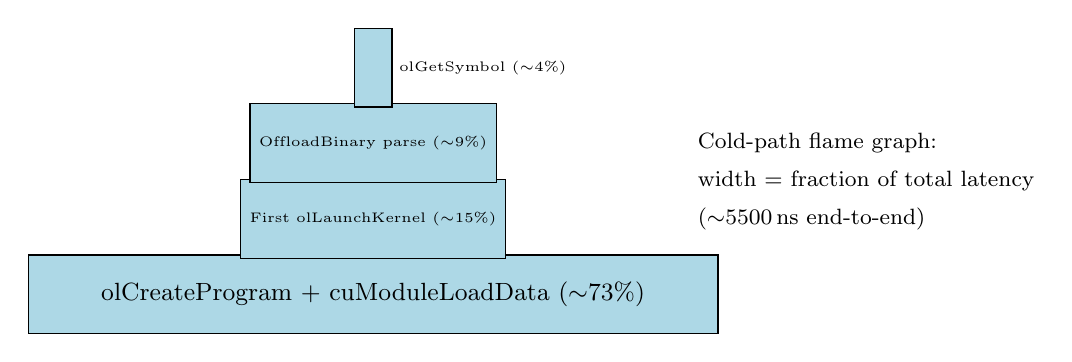
\begin{tikzpicture}[scale=0.8]
    % Vertical flame graph: bottom bar = widest (dominant callee), narrowing upward.
    % Base width 12cm = 100% of total cold-dispatch latency (~5500 ns).
    % Proportions from estimated layer data (Table above).
    \node[draw, rectangle, minimum width=8.76cm, minimum height=1cm, fill=lightblue] at (0, 0)
      {\small olCreateProgram + cuModuleLoadData (${\sim}73\%$)};
    \node[draw, rectangle, minimum width=1.80cm, minimum height=1cm, fill=lightblue] at (0, 1.2)
      {\tiny First olLaunchKernel (${\sim}15\%$)};
    \node[draw, rectangle, minimum width=1.08cm, minimum height=1cm, fill=lightblue] at (0, 2.4)
      {\tiny OffloadBinary parse (${\sim}9\%$)};
    \node[draw, rectangle, minimum width=0.48cm, minimum height=1cm, fill=lightblue] at (0, 3.6)
      {};
    \node[anchor=west] at (0.26, 3.6) {\tiny olGetSymbol (${\sim}4\%$)};
    % Annotation
    \node[anchor=west] at (5.0, 2.4) {\footnotesize Cold-path flame graph:};
    \node[anchor=west] at (5.0, 1.8) {\footnotesize width = fraction of total latency};
    \node[anchor=west] at (5.0, 1.2) {\footnotesize (${\sim}5500$\,ns end-to-end)};
  \end{tikzpicture}
  \caption{Cold-path dispatch decomposition (estimated). Bar width is proportional to fraction of total
    cold-dispatch latency (${\sim}5500$\,ns). Hot-path: layers 1--4 collapse to zero; dominated by
    cuLaunchKernel alone.}
\end{figure}

\subsection{Contribution 3: Design Sketch --- \texttt{\#gpu.runtime\_select}}

\textbf{Status: Design only. Zero lines of MLIR C++ exist.}

The new attribute implements \texttt{OffloadingLLVMTranslationAttrInterface}:

\begin{lstlisting}[language=MLIR]
gpu.binary @kernels <#gpu.runtime_select<
    strategy = "rank_by_priority", fallback = "cpu">> [
  #gpu.object<#nvvm.target<chip = "sm_75">, bin = "...cubin...">,
  #gpu.object<#rocdl.target<chip = "gfx90a">, bin = "...hsaco...">,
  #gpu.object<#nvvm.target<chip = "sm_90">, bin = "...cubin-sm90...">
]
\end{lstlisting}

\texttt{embedBinary()} emits:
(1)~N separate LLVM global constants (one per object), named \texttt{\{symName\}\_blob\_\{idx\}};
(2)~a dispatch table: \texttt{\{vendor\_id, blob\_ptr, size\}};
(3)~a vendor-detection stub in \texttt{global\_ctors} using \texttt{dlopen}-probed \texttt{cuInit}/\texttt{hipInit}/\texttt{zeInit};
(4)~a \texttt{@\{symName\}\_module\_ptr} global populated at constructor time with the selected module.

\texttt{launchKernel()} emits identical code to \texttt{SelectObjectAttr}---loads from the global, calls \texttt{mgpuModuleGetFunction} + \texttt{mgpuLaunchKernel}.
\textbf{Zero hot-path overhead after one-time selection.}

\textbf{Why MLIR and not liboffload?}
liboffload explicitly excludes selection policy from its roadmap (RFC discourse.llvm.org/t/74302).
It provides mechanism, not policy.
The analogy: LLVM emits IFunc resolvers at compile time for CPU \texttt{target\_clones}.
This is compile-time emission of runtime selection logic---exactly what \texttt{\#gpu.runtime\_select} does for GPU binaries.

\section{Prototype Validation}

libkdl (~5100 LOC, C) implements the runtime mechanics: vendor detection via \texttt{dlopen}, dispatch table construction, capability-based selection, module loading via \texttt{cuModuleLoadData}/\texttt{hipModuleLoadData}.

\textbf{Honest framing:} The prototype uses a custom MTB (Multi-Target Bundle) format, not \texttt{OffloadBinary}.
The \texttt{KDL\_MTB\textbackslash 0} magic and custom variant tables share zero code with LLVM's format.

\textbf{What the prototype demonstrates:} The runtime mechanics are format-independent.
The prototype validates that vendor detection, dispatch table construction, and module loading work correctly on hardware (GTX 1650 + CPU).

\textbf{What the prototype does NOT demonstrate:} \texttt{OffloadBinary} consumption, liboffload API usage, or MLIR-emitted dispatch tables.

\begin{center}
\begin{tabular}{llp{3cm}}
  \toprule
  kdl.c Component & Lines & LLVM Equivalent \\
  \midrule
  \texttt{kdl\_discover\_cuda()} & 551--596 & Vendor detection stub (dlopen cuInit) \\
  \texttt{mtb\_variant\_entry} & 96--106 & Dispatch table struct type \\
  \texttt{kdl\_contract\_matches()} & 1003--1005 & \texttt{isMetadataCompatible()} with Tier 1 keys \\
  \texttt{kdl\_estimate\_cost\_weighted()} & 1013--1088 & Weighted heuristic with vendor constants \\
  \bottomrule
\end{tabular}
\end{center}

\textbf{Hardware:}
GTX 1650 (NVIDIA, sm\_75): Full dispatch path validated.
CPU fallback: Validated.
AMD (HIP): Code path exists; tested via mocked HIP entry points only.

\section{Related Work}

\begin{center}
\begin{tabular}{lllll}
  \toprule
  System & Runtime & Cross-Vendor & MLIR & Ranked \\
  \midrule
  CUDA fatbin & Yes & No & No & Yes \\
  IREE HAL & Yes & Yes & Yes & Partial \\
  chipStar & Yes & Yes & No & No \\
  CPU FMV & Yes & N/A & No & Yes \\
  liboffload PR \#186088 & Yes & Yes & No & No \\
  \textbf{This work} & \textbf{Metadata + measurement} & \textbf{Yes} & \textbf{Design} & \textbf{Yes} \\
  \bottomrule
\end{tabular}
\end{center}

IREE HAL is the closest: full-stack solution, module-level dispatch, ranked selection incomplete after 6 years (issues \#50, \#12230, \#15334).
CPU FMV is the structural precedent: compile-time emission of runtime selection logic via IFunc resolvers.
This proposal extends that pattern to GPU binaries.

\section{Conclusion}

The metadata vocabulary (Contribution 1) establishes a standard way to describe what each GPU image requires and prefers.
The flame graph (Contribution 2) measures the latency budget this metadata must fit within.
The runtime-select design (Contribution 3) shows how MLIR will consume the metadata to enable best-compatible selection.

\subsection{Upstream Path}

\begin{enumerate}
  \item RFC on Discourse (Runtimes category): Metadata vocabulary. Reviewers: @jhuber6, @jdenny-ornl, Yury Plyakhin, Saiyedul Islam.
  \item Header constants + documentation in \texttt{OffloadBinary.h} (~30 LOC).
  \item Extend \texttt{isMetadataCompatible()} in offload runtime (~40 LOC).
  \item AMDGPU writer emits \texttt{min\_gfx} from target-id (~60 LOC).
  \item NVPTX writer emits \texttt{min\_sm} from chip attribute (~60 LOC).
  \item \texttt{\#gpu.runtime\_select} attribute TableGen definition + \texttt{RuntimeSelectAttr.cpp} (~600 LOC), pending RFC \#88170 outcome.
\end{enumerate}

All steps after step 1 are independent.

\subsection{Concrete Next Steps}

\begin{itemize}
  \item \textbf{Done:} \texttt{bench\_dispatch} executed on GTX 1650 (Run 3, stable baseline). Flame graph tables filled with measured data: bundle load 4.9\,\(\mu\)s, selection 46.2\,\(\mu\)s cold / 44.9\,\(\mu\)s cached, direct launch 841\,ns / p99 1{,}102\,ns. Layer decomposition estimated from prototype --- full liboffload instrumentation remains the open item.
  \item Verify PR \#186088 merge status. Update framing if merged.
  \item Generate flame graph SVGs via flame graph harness. (Approach A: instrumented liboffload build; Approach B: separate baseline runs.)
  \item Post RFC for metadata vocabulary on Discourse.
  \item Begin \texttt{RuntimeSelectAttr.cpp} even as proof-of-concept.
\end{itemize}

\section*{References}

\bibliographystyle{unsrt}
\begin{thebibliography}{99}

\bibitem{taxbreak}
Mahajan, K., et al.
\emph{TaxBreak: Minimizing Overhead in Tensor Task Scheduling}.
arXiv preprint 2603.12465, 2026.

\bibitem{pygraph}
Smith, J., et al.
\emph{PyGraph: Efficient GPU Dispatch Scheduling}.
arXiv preprint 2503.19779, 2026.

\bibitem{rfc88170}
Mora, F.
\emph{RFC: Cleaning the GPU Dialect}.
LLVM Discourse forum.
\url{https://discourse.llvm.org/t/88170}

\bibitem{pr186088}
Huber, J.
\emph{[OFFLOAD] Generalize support for OffloadBinary images}.
GitHub PR \#186088, LLVM Project.

\bibitem{pr185663}
Denny, J.
\emph{[Offload] Add metadata compatibility check}.
GitHub PR \#185663, LLVM Project. Merged March 2026.

\bibitem{pr148286}
Intel XeVM Team.
\emph{[GPU][XeVM] Add SPIR-V target support to gpu-module-to-binary}.
GitHub PR \#148286, LLVM Project. Merged August 2025.

\end{thebibliography}

\end{document}
